\documentclass[11pt,a4paper]{article}
\usepackage[utf8]{inputenc}
\usepackage[T1]{fontenc}
\usepackage{lmodern}
\usepackage[margin=2.3cm]{geometry}
\usepackage{microtype}
\usepackage{amsmath,amssymb}
\usepackage{graphicx}
\usepackage{booktabs}
\usepackage{enumitem}
\usepackage{xcolor}
\usepackage[most]{tcolorbox}
\usepackage{listings}
\usepackage[hidelinks]{hyperref}
\graphicspath{{../report/figures/}}
% Generated by model/report.py from the results files. Do not edit by hand.
\newcommand{\BaselineTrivialMeanFullTwoOneTestRmse}{41.58}
\newcommand{\BaselineTrivialMeanFullTwoOneTestRmseStd}{0.00}
\newcommand{\BaselineTrivialMeanFullTwoOneTestMae}{36.98}
\newcommand{\BaselineTrivialMeanFullTwoOneTestNasa}{302.35}
\newcommand{\BaselineTrivialMeanFullTwoOneStatusAcc}{0.717}
\newcommand{\BaselineTrivialMeanFullTwoOneStatusAccPct}{71.7}
\newcommand{\BaselineTrivialMeanFullTwoOneStatusFOne}{0.278}
\newcommand{\BaselineTrivialMeanFullTwoOneCriticalRecall}{0.000}
\newcommand{\BaselineTrivialMeanFullTwoOneOfficialRmse}{41.97}
\newcommand{\BaselineTrivialMeanFullTwoOneNEstimators}{0}
\newcommand{\BaselineTrivialMeanFullTwoOneNSensors}{21}
\newcommand{\BaselineTrivialMeanFullTwoOneTrainSeconds}{0}
\newcommand{\BaselineRidgeFullTwoOneTestRmse}{18.78}
\newcommand{\BaselineRidgeFullTwoOneTestRmseStd}{0.00}
\newcommand{\BaselineRidgeFullTwoOneTestMae}{14.26}
\newcommand{\BaselineRidgeFullTwoOneTestNasa}{7.28}
\newcommand{\BaselineRidgeFullTwoOneStatusAcc}{0.850}
\newcommand{\BaselineRidgeFullTwoOneStatusAccPct}{85.0}
\newcommand{\BaselineRidgeFullTwoOneStatusFOne}{0.700}
\newcommand{\BaselineRidgeFullTwoOneCriticalRecall}{0.640}
\newcommand{\BaselineRidgeFullTwoOneOfficialRmse}{19.45}
\newcommand{\BaselineRidgeFullTwoOneNEstimators}{0}
\newcommand{\BaselineRidgeFullTwoOneNSensors}{21}
\newcommand{\BaselineRidgeFullTwoOneTrainSeconds}{0}
\newcommand{\BaselineTrivialMeanInformativeOneFiveTestRmse}{41.58}
\newcommand{\BaselineTrivialMeanInformativeOneFiveTestRmseStd}{0.00}
\newcommand{\BaselineTrivialMeanInformativeOneFiveTestMae}{36.98}
\newcommand{\BaselineTrivialMeanInformativeOneFiveTestNasa}{302.35}
\newcommand{\BaselineTrivialMeanInformativeOneFiveStatusAcc}{0.717}
\newcommand{\BaselineTrivialMeanInformativeOneFiveStatusAccPct}{71.7}
\newcommand{\BaselineTrivialMeanInformativeOneFiveStatusFOne}{0.278}
\newcommand{\BaselineTrivialMeanInformativeOneFiveCriticalRecall}{0.000}
\newcommand{\BaselineTrivialMeanInformativeOneFiveOfficialRmse}{41.97}
\newcommand{\BaselineTrivialMeanInformativeOneFiveNEstimators}{0}
\newcommand{\BaselineTrivialMeanInformativeOneFiveNSensors}{15}
\newcommand{\BaselineTrivialMeanInformativeOneFiveTrainSeconds}{0}
\newcommand{\BaselineRidgeInformativeOneFiveTestRmse}{19.01}
\newcommand{\BaselineRidgeInformativeOneFiveTestRmseStd}{0.00}
\newcommand{\BaselineRidgeInformativeOneFiveTestMae}{14.37}
\newcommand{\BaselineRidgeInformativeOneFiveTestNasa}{7.77}
\newcommand{\BaselineRidgeInformativeOneFiveStatusAcc}{0.850}
\newcommand{\BaselineRidgeInformativeOneFiveStatusAccPct}{85.0}
\newcommand{\BaselineRidgeInformativeOneFiveStatusFOne}{0.699}
\newcommand{\BaselineRidgeInformativeOneFiveCriticalRecall}{0.638}
\newcommand{\BaselineRidgeInformativeOneFiveOfficialRmse}{19.53}
\newcommand{\BaselineRidgeInformativeOneFiveNEstimators}{0}
\newcommand{\BaselineRidgeInformativeOneFiveNSensors}{15}
\newcommand{\BaselineRidgeInformativeOneFiveTrainSeconds}{0}
\newcommand{\BaselineTrivialMeanReducedEightTestRmse}{41.58}
\newcommand{\BaselineTrivialMeanReducedEightTestRmseStd}{0.00}
\newcommand{\BaselineTrivialMeanReducedEightTestMae}{36.98}
\newcommand{\BaselineTrivialMeanReducedEightTestNasa}{302.35}
\newcommand{\BaselineTrivialMeanReducedEightStatusAcc}{0.717}
\newcommand{\BaselineTrivialMeanReducedEightStatusAccPct}{71.7}
\newcommand{\BaselineTrivialMeanReducedEightStatusFOne}{0.278}
\newcommand{\BaselineTrivialMeanReducedEightCriticalRecall}{0.000}
\newcommand{\BaselineTrivialMeanReducedEightOfficialRmse}{41.97}
\newcommand{\BaselineTrivialMeanReducedEightNEstimators}{0}
\newcommand{\BaselineTrivialMeanReducedEightNSensors}{8}
\newcommand{\BaselineTrivialMeanReducedEightTrainSeconds}{0}
\newcommand{\BaselineRidgeReducedEightTestRmse}{20.86}
\newcommand{\BaselineRidgeReducedEightTestRmseStd}{0.00}
\newcommand{\BaselineRidgeReducedEightTestMae}{15.61}
\newcommand{\BaselineRidgeReducedEightTestNasa}{9.21}
\newcommand{\BaselineRidgeReducedEightStatusAcc}{0.849}
\newcommand{\BaselineRidgeReducedEightStatusAccPct}{84.9}
\newcommand{\BaselineRidgeReducedEightStatusFOne}{0.695}
\newcommand{\BaselineRidgeReducedEightCriticalRecall}{0.616}
\newcommand{\BaselineRidgeReducedEightOfficialRmse}{21.33}
\newcommand{\BaselineRidgeReducedEightNEstimators}{0}
\newcommand{\BaselineRidgeReducedEightNSensors}{8}
\newcommand{\BaselineRidgeReducedEightTrainSeconds}{0}
\newcommand{\MainGbrFullTwoOneTestRmse}{12.99}
\newcommand{\MainGbrFullTwoOneTestRmseStd}{0.07}
\newcommand{\MainGbrFullTwoOneTestMae}{9.40}
\newcommand{\MainGbrFullTwoOneTestNasa}{2.86}
\newcommand{\MainGbrFullTwoOneStatusAcc}{0.921}
\newcommand{\MainGbrFullTwoOneStatusAccPct}{92.1}
\newcommand{\MainGbrFullTwoOneStatusFOne}{0.845}
\newcommand{\MainGbrFullTwoOneCriticalRecall}{0.933}
\newcommand{\MainGbrFullTwoOneOfficialRmse}{13.22}
\newcommand{\MainGbrFullTwoOneNEstimators}{200}
\newcommand{\MainGbrFullTwoOneNSensors}{21}
\newcommand{\MainGbrFullTwoOneTrainSeconds}{245}
\newcommand{\MainGbrInformativeOneFiveTestRmse}{12.99}
\newcommand{\MainGbrInformativeOneFiveTestRmseStd}{0.07}
\newcommand{\MainGbrInformativeOneFiveTestMae}{9.40}
\newcommand{\MainGbrInformativeOneFiveTestNasa}{2.86}
\newcommand{\MainGbrInformativeOneFiveStatusAcc}{0.921}
\newcommand{\MainGbrInformativeOneFiveStatusAccPct}{92.1}
\newcommand{\MainGbrInformativeOneFiveStatusFOne}{0.845}
\newcommand{\MainGbrInformativeOneFiveCriticalRecall}{0.933}
\newcommand{\MainGbrInformativeOneFiveOfficialRmse}{13.22}
\newcommand{\MainGbrInformativeOneFiveNEstimators}{200}
\newcommand{\MainGbrInformativeOneFiveNSensors}{15}
\newcommand{\MainGbrInformativeOneFiveTrainSeconds}{255}
\newcommand{\MainGbrReducedEightTestRmse}{15.56}
\newcommand{\MainGbrReducedEightTestRmseStd}{0.06}
\newcommand{\MainGbrReducedEightTestMae}{11.15}
\newcommand{\MainGbrReducedEightTestNasa}{4.35}
\newcommand{\MainGbrReducedEightStatusAcc}{0.913}
\newcommand{\MainGbrReducedEightStatusAccPct}{91.3}
\newcommand{\MainGbrReducedEightStatusFOne}{0.832}
\newcommand{\MainGbrReducedEightCriticalRecall}{0.935}
\newcommand{\MainGbrReducedEightOfficialRmse}{15.35}
\newcommand{\MainGbrReducedEightNEstimators}{300}
\newcommand{\MainGbrReducedEightNSensors}{8}
\newcommand{\MainGbrReducedEightTrainSeconds}{136}
\newcommand{\PosthocGbrGreedyEightTestRmse}{13.88}
\newcommand{\PosthocGbrGreedyEightTestRmseStd}{0.12}
\newcommand{\PosthocGbrGreedyEightTestMae}{9.88}
\newcommand{\PosthocGbrGreedyEightTestNasa}{3.34}
\newcommand{\PosthocGbrGreedyEightStatusAcc}{0.918}
\newcommand{\PosthocGbrGreedyEightStatusAccPct}{91.8}
\newcommand{\PosthocGbrGreedyEightStatusFOne}{0.844}
\newcommand{\PosthocGbrGreedyEightCriticalRecall}{0.932}
\newcommand{\PosthocGbrGreedyEightOfficialRmse}{13.20}
\newcommand{\PosthocGbrGreedyEightNEstimators}{300}
\newcommand{\PosthocGbrGreedyEightNSensors}{8}
\newcommand{\PosthocGbrGreedyEightTrainSeconds}{115}
\newcommand{\PosthocGbrFullTwoOneWOneZeroTestRmse}{17.79}
\newcommand{\PosthocGbrFullTwoOneWOneZeroTestRmseStd}{0.04}
\newcommand{\PosthocGbrFullTwoOneWOneZeroTestMae}{12.61}
\newcommand{\PosthocGbrFullTwoOneWOneZeroTestNasa}{11.63}
\newcommand{\PosthocGbrFullTwoOneWOneZeroStatusAcc}{0.891}
\newcommand{\PosthocGbrFullTwoOneWOneZeroStatusAccPct}{89.1}
\newcommand{\PosthocGbrFullTwoOneWOneZeroStatusFOne}{0.794}
\newcommand{\PosthocGbrFullTwoOneWOneZeroCriticalRecall}{0.851}
\newcommand{\PosthocGbrFullTwoOneWOneZeroOfficialRmse}{18.13}
\newcommand{\PosthocGbrFullTwoOneWOneZeroNEstimators}{200}
\newcommand{\PosthocGbrFullTwoOneWOneZeroNSensors}{21}
\newcommand{\PosthocGbrFullTwoOneWOneZeroTrainSeconds}{184}
\newcommand{\PosthocGbrReducedEightWOneZeroTestRmse}{19.01}
\newcommand{\PosthocGbrReducedEightWOneZeroTestRmseStd}{0.04}
\newcommand{\PosthocGbrReducedEightWOneZeroTestMae}{14.24}
\newcommand{\PosthocGbrReducedEightWOneZeroTestNasa}{11.31}
\newcommand{\PosthocGbrReducedEightWOneZeroStatusAcc}{0.874}
\newcommand{\PosthocGbrReducedEightWOneZeroStatusAccPct}{87.4}
\newcommand{\PosthocGbrReducedEightWOneZeroStatusFOne}{0.749}
\newcommand{\PosthocGbrReducedEightWOneZeroCriticalRecall}{0.814}
\newcommand{\PosthocGbrReducedEightWOneZeroOfficialRmse}{19.71}
\newcommand{\PosthocGbrReducedEightWOneZeroNEstimators}{200}
\newcommand{\PosthocGbrReducedEightWOneZeroNSensors}{8}
\newcommand{\PosthocGbrReducedEightWOneZeroTrainSeconds}{108}
\newcommand{\PosthocGbrFullTwoOneWSixZeroTestRmse}{11.16}
\newcommand{\PosthocGbrFullTwoOneWSixZeroTestRmseStd}{0.11}
\newcommand{\PosthocGbrFullTwoOneWSixZeroTestMae}{8.07}
\newcommand{\PosthocGbrFullTwoOneWSixZeroTestNasa}{1.96}
\newcommand{\PosthocGbrFullTwoOneWSixZeroStatusAcc}{0.932}
\newcommand{\PosthocGbrFullTwoOneWSixZeroStatusAccPct}{93.2}
\newcommand{\PosthocGbrFullTwoOneWSixZeroStatusFOne}{0.880}
\newcommand{\PosthocGbrFullTwoOneWSixZeroCriticalRecall}{0.921}
\newcommand{\PosthocGbrFullTwoOneWSixZeroOfficialRmse}{12.67}
\newcommand{\PosthocGbrFullTwoOneWSixZeroNEstimators}{800}
\newcommand{\PosthocGbrFullTwoOneWSixZeroNSensors}{21}
\newcommand{\PosthocGbrFullTwoOneWSixZeroTrainSeconds}{201}
\newcommand{\PosthocGbrReducedEightWSixZeroTestRmse}{12.91}
\newcommand{\PosthocGbrReducedEightWSixZeroTestRmseStd}{0.01}
\newcommand{\PosthocGbrReducedEightWSixZeroTestMae}{9.35}
\newcommand{\PosthocGbrReducedEightWSixZeroTestNasa}{2.51}
\newcommand{\PosthocGbrReducedEightWSixZeroStatusAcc}{0.925}
\newcommand{\PosthocGbrReducedEightWSixZeroStatusAccPct}{92.5}
\newcommand{\PosthocGbrReducedEightWSixZeroStatusFOne}{0.871}
\newcommand{\PosthocGbrReducedEightWSixZeroCriticalRecall}{0.956}
\newcommand{\PosthocGbrReducedEightWSixZeroOfficialRmse}{14.07}
\newcommand{\PosthocGbrReducedEightWSixZeroNEstimators}{300}
\newcommand{\PosthocGbrReducedEightWSixZeroNSensors}{8}
\newcommand{\PosthocGbrReducedEightWSixZeroTrainSeconds}{124}
\newcommand{\PosthocGbrRandomEightZeroTestRmse}{15.58}
\newcommand{\PosthocGbrRandomEightZeroTestRmseStd}{0.06}
\newcommand{\PosthocGbrRandomEightZeroTestMae}{11.16}
\newcommand{\PosthocGbrRandomEightZeroTestNasa}{5.12}
\newcommand{\PosthocGbrRandomEightZeroStatusAcc}{0.903}
\newcommand{\PosthocGbrRandomEightZeroStatusAccPct}{90.3}
\newcommand{\PosthocGbrRandomEightZeroStatusFOne}{0.812}
\newcommand{\PosthocGbrRandomEightZeroCriticalRecall}{0.886}
\newcommand{\PosthocGbrRandomEightZeroOfficialRmse}{14.43}
\newcommand{\PosthocGbrRandomEightZeroNEstimators}{200}
\newcommand{\PosthocGbrRandomEightZeroNSensors}{8}
\newcommand{\PosthocGbrRandomEightZeroTrainSeconds}{107}
\newcommand{\PosthocGbrRandomEightOneTestRmse}{13.81}
\newcommand{\PosthocGbrRandomEightOneTestRmseStd}{0.08}
\newcommand{\PosthocGbrRandomEightOneTestMae}{9.88}
\newcommand{\PosthocGbrRandomEightOneTestNasa}{3.86}
\newcommand{\PosthocGbrRandomEightOneStatusAcc}{0.922}
\newcommand{\PosthocGbrRandomEightOneStatusAccPct}{92.2}
\newcommand{\PosthocGbrRandomEightOneStatusFOne}{0.854}
\newcommand{\PosthocGbrRandomEightOneCriticalRecall}{0.924}
\newcommand{\PosthocGbrRandomEightOneOfficialRmse}{14.52}
\newcommand{\PosthocGbrRandomEightOneNEstimators}{200}
\newcommand{\PosthocGbrRandomEightOneNSensors}{8}
\newcommand{\PosthocGbrRandomEightOneTrainSeconds}{116}
\newcommand{\PosthocGbrRandomEightTwoTestRmse}{14.81}
\newcommand{\PosthocGbrRandomEightTwoTestRmseStd}{0.05}
\newcommand{\PosthocGbrRandomEightTwoTestMae}{10.97}
\newcommand{\PosthocGbrRandomEightTwoTestNasa}{4.19}
\newcommand{\PosthocGbrRandomEightTwoStatusAcc}{0.902}
\newcommand{\PosthocGbrRandomEightTwoStatusAccPct}{90.2}
\newcommand{\PosthocGbrRandomEightTwoStatusFOne}{0.808}
\newcommand{\PosthocGbrRandomEightTwoCriticalRecall}{0.886}
\newcommand{\PosthocGbrRandomEightTwoOfficialRmse}{15.36}
\newcommand{\PosthocGbrRandomEightTwoNEstimators}{100}
\newcommand{\PosthocGbrRandomEightTwoNSensors}{8}
\newcommand{\PosthocGbrRandomEightTwoTrainSeconds}{103}
\newcommand{\PosthocGbrWorstEightTestRmse}{13.96}
\newcommand{\PosthocGbrWorstEightTestRmseStd}{0.07}
\newcommand{\PosthocGbrWorstEightTestMae}{10.05}
\newcommand{\PosthocGbrWorstEightTestNasa}{3.90}
\newcommand{\PosthocGbrWorstEightStatusAcc}{0.917}
\newcommand{\PosthocGbrWorstEightStatusAccPct}{91.7}
\newcommand{\PosthocGbrWorstEightStatusFOne}{0.843}
\newcommand{\PosthocGbrWorstEightCriticalRecall}{0.910}
\newcommand{\PosthocGbrWorstEightOfficialRmse}{14.08}
\newcommand{\PosthocGbrWorstEightNEstimators}{200}
\newcommand{\PosthocGbrWorstEightNSensors}{8}
\newcommand{\PosthocGbrWorstEightTrainSeconds}{5003}
\newcommand{\PosthocGbrFullTwoOneRowsplitTestRmse}{10.08}
\newcommand{\PosthocGbrFullTwoOneRowsplitTestRmseStd}{0.27}
\newcommand{\PosthocGbrFullTwoOneRowsplitTestMae}{7.06}
\newcommand{\PosthocGbrFullTwoOneRowsplitTestNasa}{1.63}
\newcommand{\PosthocGbrFullTwoOneRowsplitStatusAcc}{0.934}
\newcommand{\PosthocGbrFullTwoOneRowsplitStatusAccPct}{93.4}
\newcommand{\PosthocGbrFullTwoOneRowsplitStatusFOne}{0.884}
\newcommand{\PosthocGbrFullTwoOneRowsplitCriticalRecall}{0.921}
\newcommand{\PosthocGbrFullTwoOneRowsplitOfficialRmse}{13.54}
\newcommand{\PosthocGbrFullTwoOneRowsplitNEstimators}{200}
\newcommand{\PosthocGbrFullTwoOneRowsplitNSensors}{21}
\newcommand{\PosthocGbrFullTwoOneRowsplitTrainSeconds}{63}
\newcommand{\PosthocGbrFullTwoOneCapOneZeroZeroTestRmse}{8.42}
\newcommand{\PosthocGbrFullTwoOneCapOneZeroZeroTestRmseStd}{0.06}
\newcommand{\PosthocGbrFullTwoOneCapOneZeroZeroTestMae}{5.60}
\newcommand{\PosthocGbrFullTwoOneCapOneZeroZeroTestNasa}{1.14}
\newcommand{\PosthocGbrFullTwoOneCapOneZeroZeroStatusAcc}{0.923}
\newcommand{\PosthocGbrFullTwoOneCapOneZeroZeroStatusAccPct}{92.3}
\newcommand{\PosthocGbrFullTwoOneCapOneZeroZeroStatusFOne}{0.855}
\newcommand{\PosthocGbrFullTwoOneCapOneZeroZeroCriticalRecall}{0.930}
\newcommand{\PosthocGbrFullTwoOneCapOneZeroZeroOfficialRmse}{9.40}
\newcommand{\PosthocGbrFullTwoOneCapOneZeroZeroNEstimators}{200}
\newcommand{\PosthocGbrFullTwoOneCapOneZeroZeroNSensors}{21}
\newcommand{\PosthocGbrFullTwoOneCapOneZeroZeroTrainSeconds}{240}
\newcommand{\PosthocGbrReducedEightCapOneZeroZeroTestRmse}{10.26}
\newcommand{\PosthocGbrReducedEightCapOneZeroZeroTestRmseStd}{0.10}
\newcommand{\PosthocGbrReducedEightCapOneZeroZeroTestMae}{6.83}
\newcommand{\PosthocGbrReducedEightCapOneZeroZeroTestNasa}{1.57}
\newcommand{\PosthocGbrReducedEightCapOneZeroZeroStatusAcc}{0.919}
\newcommand{\PosthocGbrReducedEightCapOneZeroZeroStatusAccPct}{91.9}
\newcommand{\PosthocGbrReducedEightCapOneZeroZeroStatusFOne}{0.846}
\newcommand{\PosthocGbrReducedEightCapOneZeroZeroCriticalRecall}{0.933}
\newcommand{\PosthocGbrReducedEightCapOneZeroZeroOfficialRmse}{11.59}
\newcommand{\PosthocGbrReducedEightCapOneZeroZeroNEstimators}{400}
\newcommand{\PosthocGbrReducedEightCapOneZeroZeroNSensors}{8}
\newcommand{\PosthocGbrReducedEightCapOneZeroZeroTrainSeconds}{135}
\newcommand{\PosthocGbrFullTwoOneCapOneFiveZeroTestRmse}{19.14}
\newcommand{\PosthocGbrFullTwoOneCapOneFiveZeroTestRmseStd}{0.05}
\newcommand{\PosthocGbrFullTwoOneCapOneFiveZeroTestMae}{14.49}
\newcommand{\PosthocGbrFullTwoOneCapOneFiveZeroTestNasa}{8.50}
\newcommand{\PosthocGbrFullTwoOneCapOneFiveZeroStatusAcc}{0.912}
\newcommand{\PosthocGbrFullTwoOneCapOneFiveZeroStatusAccPct}{91.2}
\newcommand{\PosthocGbrFullTwoOneCapOneFiveZeroStatusFOne}{0.826}
\newcommand{\PosthocGbrFullTwoOneCapOneFiveZeroCriticalRecall}{0.926}
\newcommand{\PosthocGbrFullTwoOneCapOneFiveZeroOfficialRmse}{17.98}
\newcommand{\PosthocGbrFullTwoOneCapOneFiveZeroNEstimators}{300}
\newcommand{\PosthocGbrFullTwoOneCapOneFiveZeroNSensors}{21}
\newcommand{\PosthocGbrFullTwoOneCapOneFiveZeroTrainSeconds}{230}
\newcommand{\PosthocGbrReducedEightCapOneFiveZeroTestRmse}{21.35}
\newcommand{\PosthocGbrReducedEightCapOneFiveZeroTestRmseStd}{0.12}
\newcommand{\PosthocGbrReducedEightCapOneFiveZeroTestMae}{16.11}
\newcommand{\PosthocGbrReducedEightCapOneFiveZeroTestNasa}{12.82}
\newcommand{\PosthocGbrReducedEightCapOneFiveZeroStatusAcc}{0.909}
\newcommand{\PosthocGbrReducedEightCapOneFiveZeroStatusAccPct}{90.9}
\newcommand{\PosthocGbrReducedEightCapOneFiveZeroStatusFOne}{0.821}
\newcommand{\PosthocGbrReducedEightCapOneFiveZeroCriticalRecall}{0.919}
\newcommand{\PosthocGbrReducedEightCapOneFiveZeroOfficialRmse}{19.23}
\newcommand{\PosthocGbrReducedEightCapOneFiveZeroNEstimators}{200}
\newcommand{\PosthocGbrReducedEightCapOneFiveZeroNSensors}{8}
\newcommand{\PosthocGbrReducedEightCapOneFiveZeroTrainSeconds}{130}
\newcommand{\Margin}{1.0}
\newcommand{\HypGap}{2.57}
\newcommand{\HypGapMin}{2.49}
\newcommand{\HypGapMax}{2.68}
\newcommand{\HypHolds}{no}
\newcommand{\DeployedArm}{full21}
\newcommand{\TrivOverGbr}{3.2}
\newcommand{\GreedyEightGap}{0.89}
\newcommand{\WorstEightGap}{0.97}
\newcommand{\RandomEightTestRmse}{14.74}
\newcommand{\RandomEightTestRmseStd}{0.77}
\newcommand{\RandomEightGap}{1.75}
\newcommand{\RandomEightDraws}{3}
\newcommand{\GapWOneZero}{1.22}
\newcommand{\GapWSixZero}{1.75}
\newcommand{\GapCapOneZeroZero}{1.84}
\newcommand{\GapCapOneFiveZero}{2.21}
\newcommand{\WindowEffectFullTwoOne}{1.83}
\newcommand{\RowsplitRmse}{10.08}
\newcommand{\RowsplitOptimism}{2.91}
\newcommand{\RowsplitOptimismPct}{22}
\newcommand{\GreedyEightSensors}{8, 9, 11, 12, 13, 14, 17, 20}
\newcommand{\ReducedEightSensors}{2, 3, 4, 11, 15, 17, 20, 21}
\newcommand{\InformativeSensors}{2, 3, 4, 6, 7, 8, 9, 11, 12, 13, 14, 15, 17, 20, 21}
\newcommand{\ConstantSensors}{1, 5, 10, 16, 18, 19}
\newcommand{\BootFullTwoOneCiLow}{11.19}
\newcommand{\BootFullTwoOneCiHigh}{14.65}
\newcommand{\BootCiOverSeed}{26}
\newcommand{\BootDraws}{10000}
\newcommand{\BootReducedEightGapLow}{1.24}
\newcommand{\BootReducedEightGapHigh}{3.89}
\newcommand{\BootReducedEightBelowMarginPct}{1}
\newcommand{\BootGreedyEightGapLow}{$-$0.05}
\newcommand{\BootGreedyEightGapHigh}{1.96}
\newcommand{\BootGreedyEightBelowMarginPct}{62}
\newcommand{\BootWorstEightGapLow}{$-$0.28}
\newcommand{\BootWorstEightGapHigh}{2.14}
\newcommand{\BootWorstEightBelowMarginPct}{53}
\newcommand{\BootGreedyEightVsRanked}{$-$1.68}
\newcommand{\BootGreedyEightVsRankedLow}{$-$3.69}
\newcommand{\BootGreedyEightVsRankedHigh}{0.52}
\newcommand{\BootGreedyEightBetterThanRanked}{no}
\newcommand{\BootWorstEightVsRanked}{$-$1.60}
\newcommand{\BootWorstEightVsRankedLow}{$-$3.98}
\newcommand{\BootWorstEightVsRankedHigh}{0.82}
\newcommand{\BootWorstEightBetterThanRanked}{no}
\newcommand{\RedundancyReducedEight}{0.97}
\newcommand{\RedundancyWorstEight}{0.52}
\newcommand{\RedundancyGreedyEight}{0.62}
\newcommand{\RedundancyInformativeOneFive}{0.71}
\newcommand{\ConfigAuditVerdict}{recipe unchanged}
\newcommand{\ConfigAuditChanged}{deployment\_rule, onnx}
\newcommand{\ConfigAuditAffecting}{0}
\newcommand{\MainConfigHashes}{0b24782979f5 (full21); 838cd9be81f5 (informative15, reduced8)}
\newcommand{\NMainConfigHashes}{2}
\newcommand{\RandomEightBestGap}{0.83}
\newcommand{\RandomEightWorstGap}{2.60}
\newcommand{\SplitTrain}{70}
\newcommand{\SplitVal}{15}
\newcommand{\SplitTest}{15}
\newcommand{\CfgLearningRate}{0.05}
\newcommand{\CfgMaxDepth}{4}
\newcommand{\CfgSubsample}{0.8}
\newcommand{\CfgGridMin}{100}
\newcommand{\CfgGridMax}{800}
\newcommand{\CfgFeaturesFull}{63}
\newcommand{\CfgParityTolExp}{-3}
\newcommand{\CfgFeatureTolExp}{-6}
\newcommand{\AlertWarningBelow}{60}
\newcommand{\AlertCriticalBelow}{30}
\newcommand{\AlertTrendWindow}{30}
\newcommand{\AlertTrendSlope}{$-$2.0}
\newcommand{\AlertTrendClearSlope}{$-$1.5}
\newcommand{\AlertMinWindowRows}{30}
\newcommand{\AlertCloseAfter}{5}
\newcommand{\AlertHysteresis}{10}
\newcommand{\ParityRows}{300}
\newcommand{\OriginalTrendDrop}{20}
\newcommand{\OriginalTrendWindow}{10}
\newcommand{\NRunsTotal}{57}
\newcommand{\NRunsMain}{9}
\newcommand{\NRunsPosthoc}{42}
\newcommand{\ConfigHash}{0b24782979f5}
\newcommand{\Window}{30}
\newcommand{\LabelCap}{125}
\newcommand{\NSeeds}{3}
\newcommand{\EdaRows}{20631}
\newcommand{\EdaEngines}{100}
\newcommand{\EdaLifeMin}{128}
\newcommand{\EdaLifeMax}{362}
\newcommand{\EdaLifeMedian}{199}
\newcommand{\EdaShareRowsAboveCap}{38.9}
\newcommand{\AuditConstSplits}{0}
\newcommand{\AuditImportanceOutsidePct}{19.5}
\newcommand{\AuditTopOutside}{9, 12, 14, 7}
\newcommand{\AlertReplayValEngines}{15}
\newcommand{\AlertReplayValEnginesPassing}{15}
\newcommand{\AlertReplayValAlertsTotal}{30}
\newcommand{\AlertReplayValMeanTrueRulAtWarning}{56.7}
\newcommand{\AlertReplayValMinTrueRulAtWarning}{38}
\newcommand{\AlertReplayValMeanTrueRulAtCritical}{29.0}
\newcommand{\AlertReplayValMinTrueRulAtCritical}{19}
\newcommand{\AlertReplayTestEngines}{15}
\newcommand{\AlertReplayTestEnginesPassing}{15}
\newcommand{\AlertReplayTestAlertsTotal}{30}
\newcommand{\AlertReplayTestMeanTrueRulAtWarning}{54.5}
\newcommand{\AlertReplayTestMinTrueRulAtWarning}{40}
\newcommand{\AlertReplayTestMeanTrueRulAtCritical}{31.7}
\newcommand{\AlertReplayTestMinTrueRulAtCritical}{21}
\newcommand{\AlertOriginalPass}{2}
\newcommand{\AlertOriginalAlerts}{59}
\newcommand{\AlertChosenPass}{15}
\newcommand{\RestartFileRows}{20631}
\newcommand{\RestartReadingsRows}{20631}
\newcommand{\RestartHealthScoresRows}{20631}
\newcommand{\RestartMachinesScoredExactlyOneToLife}{100}
\newcommand{\RestartMachines}{100}
\newcommand{\RestartRedeliveredAndIgnoredAsLate}{2}
\newcommand{\RestartFinalConsumerLag}{0}
\newcommand{\RestartMachinesWithAlertsDifferentFromUninterruptedRun}{0}
\newcommand{\RestartMachinesWithRepeatedAlertOfOneSeverity}{4}
\newcommand{\RestartMaxDiff}{9e$-$05}
\newcommand{\RestartSecondsDown}{24.5}
\newcommand{\RestartPeakLag}{11175}
\newcommand{\RestartReadingsWhileDown}{6585}
\newcommand{\RestartPassed}{yes}
\newcommand{\AllEnginesAlertPass}{96}
\newcommand{\EaTestRows}{3183}
\newcommand{\EaMisclassifiedRows}{248}
\newcommand{\EaInspected}{35}
\newcommand{\EaAmbiguous}{3}
\newcommand{\EaMislabeled}{0}
\newcommand{\EaModel}{32}
\newcommand{\EaTopConfusionRows}{135}
\newcommand{\EaSecondConfusionRows}{58}
\newcommand{\EaHealthyAsCriticalRows}{0}
\newcommand{\EaCriticalAsHealthyRows}{0}
\newcommand{\EaMisclassifiedPct}{7.8}
\newcommand{\EaSmallErrorPct}{27}
\newcommand{\EaPatternLagging}{16}
\newcommand{\EaPatternJitter}{8}
\newcommand{\EaPatternEarly}{8}
\newcommand{\EaPatternPlateau}{2}
\newcommand{\EaPatternBoundary}{1}
\newcommand{\LtBeforeRps}{4138}
\newcommand{\LtBeforePFiveZero}{9.8}
\newcommand{\LtBeforePNineFive}{22.8}
\newcommand{\LtBeforePNineNine}{37.5}
\newcommand{\LtBeforeVus}{50}
\newcommand{\LtBeforeBatch}{1}
\newcommand{\LtBeforePoolPending}{30.4}
\newcommand{\LtBeforeDurationS}{60}
\newcommand{\LtBeforePoolPendingMax}{40}
\newcommand{\LtBeforeCpuPct}{41}
\newcommand{\LtBeforeProcessingMs}{0.97}
\newcommand{\LtBeforeInferenceMs}{0.13}
\newcommand{\LtBeforeDrainS}{0.3}
\newcommand{\LtBeforeScored}{239915}
\newcommand{\LtBeforeProcessedRps}{4115}
\newcommand{\LtBeforeRpsStd}{133}
\newcommand{\LtBeforePNineFiveStd}{0.4}
\newcommand{\LtBeforePNineNineStd}{1.7}
\newcommand{\LtBeforeRuns}{3}
\newcommand{\LtBeforePool}{10}
\newcommand{\LtAfterRps}{4318}
\newcommand{\LtAfterPFiveZero}{7.9}
\newcommand{\LtAfterPNineFive}{22.7}
\newcommand{\LtAfterPNineNine}{38.6}
\newcommand{\LtAfterVus}{50}
\newcommand{\LtAfterBatch}{1}
\newcommand{\LtAfterPoolPending}{1.3}
\newcommand{\LtAfterDurationS}{60}
\newcommand{\LtAfterPoolPendingMax}{10}
\newcommand{\LtAfterCpuPct}{41}
\newcommand{\LtAfterProcessingMs}{2.70}
\newcommand{\LtAfterInferenceMs}{0.14}
\newcommand{\LtAfterDrainS}{0.3}
\newcommand{\LtAfterScored}{235615}
\newcommand{\LtAfterProcessedRps}{4297}
\newcommand{\LtAfterRpsStd}{382}
\newcommand{\LtAfterPNineFiveStd}{1.9}
\newcommand{\LtAfterPNineNineStd}{4.6}
\newcommand{\LtAfterRuns}{3}
\newcommand{\LtAfterPool}{40}
\newcommand{\LtAfterCacheRps}{4550}
\newcommand{\LtAfterCachePFiveZero}{7.5}
\newcommand{\LtAfterCachePNineFive}{21.9}
\newcommand{\LtAfterCachePNineNine}{38.1}
\newcommand{\LtAfterCacheVus}{50}
\newcommand{\LtAfterCacheBatch}{1}
\newcommand{\LtAfterCachePoolPending}{1.3}
\newcommand{\LtAfterCacheDurationS}{60}
\newcommand{\LtAfterCachePoolPendingMax}{10}
\newcommand{\LtAfterCacheCpuPct}{40}
\newcommand{\LtAfterCacheProcessingMs}{2.86}
\newcommand{\LtAfterCacheInferenceMs}{0.14}
\newcommand{\LtAfterCacheDrainS}{0.3}
\newcommand{\LtAfterCacheScored}{245086}
\newcommand{\LtAfterCacheProcessedRps}{4528}
\newcommand{\LtAfterCacheRpsStd}{516}
\newcommand{\LtAfterCachePNineFiveStd}{2.5}
\newcommand{\LtAfterCachePNineNineStd}{6.3}
\newcommand{\LtAfterCacheRuns}{3}
\newcommand{\LtAfterCachePool}{40}
\newcommand{\LtKafkaRps}{4036}
\newcommand{\LtKafkaPFiveZero}{8.5}
\newcommand{\LtKafkaPNineFive}{24.3}
\newcommand{\LtKafkaPNineNine}{41.4}
\newcommand{\LtKafkaVus}{50}
\newcommand{\LtKafkaBatch}{1}
\newcommand{\LtKafkaPoolPending}{3.6}
\newcommand{\LtKafkaDurationS}{60}
\newcommand{\LtKafkaPoolPendingMax}{15}
\newcommand{\LtKafkaCpuPct}{38}
\newcommand{\LtKafkaProcessingMs}{1.64}
\newcommand{\LtKafkaInferenceMs}{0.14}
\newcommand{\LtKafkaDrainS}{64.9}
\newcommand{\LtKafkaScored}{214004}
\newcommand{\LtKafkaProcessedRps}{1938}
\newcommand{\LtKafkaRpsStd}{456}
\newcommand{\LtKafkaPNineFiveStd}{2.1}
\newcommand{\LtKafkaPNineNineStd}{5.9}
\newcommand{\LtKafkaRuns}{3}
\newcommand{\LtKafkaPool}{40}
\newcommand{\LtGainPct}{4}
\newcommand{\LtPoolGainMin}{$-$5}
\newcommand{\LtPoolGainMax}{10}
\newcommand{\LtPoolGainPositive}{2}
\newcommand{\LtPoolGainBlocks}{3}
\newcommand{\LtCacheGainMin}{3}
\newcommand{\LtCacheGainMax}{9}
\newcommand{\LtCacheGainPositive}{3}
\newcommand{\LtCacheGainBlocks}{3}
\newcommand{\LtTotalGainMin}{$-$2}
\newcommand{\LtTotalGainMax}{20}
\newcommand{\LtTotalGainPositive}{2}
\newcommand{\LtTotalGainBlocks}{3}
\newcommand{\LtPoolWaitsAllRunsMaxAfter}{4.4}
\newcommand{\LtPoolWaitsAllRunsMinBefore}{29.2}
\newcommand{\LtCacheGainPct}{5}
\newcommand{\LtTotalGainPct}{10}
\newcommand{\LtBestLabel}{after-cache}
\newcommand{\LtBestRps}{4550}
\newcommand{\LtBestPNineFive}{21.9}
\newcommand{\LtBestPNineNine}{38.1}
\newcommand{\JavaUsPerPrediction}{69.5}
\newcommand{\JavaPredictionsTimed}{5000}
\newcommand{\CoverageProcessingAlerts}{92.1}
\newcommand{\CoverageOverall}{91.6}
\newcommand{\CoverageRoot}{33.3}
\newcommand{\CoverageAlerts}{92.9}
\newcommand{\CoverageConfig}{96.6}
\newcommand{\CoverageIngest}{91.0}
\newcommand{\CoverageMachines}{91.1}
\newcommand{\CoverageModel}{93.9}
\newcommand{\CoverageProcessing}{91.5}
\newcommand{\CoverageQuery}{91.0}
\newcommand{\CoverageStream}{86.5}
\newcommand{\TestsJava}{58}
\newcommand{\TestsJavaFailed}{0}
\newcommand{\TestsPython}{16}
\newcommand{\TestsPythonFailed}{0}
\newcommand{\TestsPythonSkipped}{0}

\setlength{\parskip}{0.45em}
\setlength{\parindent}{0pt}
\setlist{itemsep=0.15em,topsep=0.3em}
\definecolor{mistake}{HTML}{D03B3B}
\definecolor{idea}{HTML}{2A78D6}
\newtcolorbox{mistake}[1]{colback=mistake!4,colframe=mistake!70!black,fonttitle=\bfseries,title={Mistake we caught: #1},breakable}
\newtcolorbox{keyidea}[1]{colback=idea!4,colframe=idea!70!black,fonttitle=\bfseries,title={Key idea: #1},breakable}
\lstset{basicstyle=\ttfamily\small,breaklines=true,columns=fullflexible,frame=single,framerule=0.3pt,rulecolor=\color{gray!50}}
\newcommand{\pmsd}[2]{#1\,$\pm$\,#2}
\hyphenation{Post-gre-SQL Micro-meter Test-containers}

\title{\textbf{Learn: building a real-time equipment monitor from scratch}\\[0.4em]
\large The domain, the tools, the machine learning, the evaluation,\\and every mistake made on the way}
\author{equipment-health-monitor}
\date{}

\begin{document}
\maketitle
\begin{abstract}
This tutorial explains, from first principles, everything needed to understand and rebuild the
\texttt{equipment-health-monitor} project: a Java service that scores the health of turbofan engines from a stream
of sensor readings and raises alerts. It assumes you can program; it does not assume you know predictive
maintenance, Spring, Kafka, gradient boosting or experimental design. Every number in it is generated from the
project's results files, so it can never disagree with the code.
\end{abstract}
\tableofcontents
\newpage

%=====================================================================
\section{The domain: engines, degradation and remaining useful life}

\subsection{What is being monitored}
A turbofan engine compresses air, burns fuel in it and expands the hot gas through turbines. Its parts wear:
blades erode, seals leak, clearances grow. Wear changes how the engine runs long before it fails. Temperatures
rise a little, pressures shift and fuel flow creeps up. Sensors measure these quantities every flight.
\emph{Predictive maintenance} uses those measurements to service an engine shortly before it would fail, rather
than on a fixed calendar (wasteful) or after it fails (dangerous).

\subsection{Remaining useful life}
The \emph{remaining useful life} (RUL) of an engine at a given cycle is the number of cycles it has left before
failure. A \emph{cycle} is one flight. If an engine fails after cycle 192, then at cycle 150 its RUL is 42. The
model's job is to predict RUL from the sensors seen so far.

\subsection{The data: NASA C-MAPSS}
Real run-to-failure data from real engines is rare and confidential. NASA built a detailed simulator, C-MAPSS,
and published run-to-failure trajectories from it. Each simulated engine starts with its own unknown initial
wear and manufacturing variation, then develops a fault that grows until failure. Be precise when you talk
about it: it is \emph{a NASA benchmark dataset from a physics-based simulation}, not real engine data.

We use subset FD001: one operating condition (sea level) and one fault mode (high-pressure compressor
degradation). The training file has \EdaEngines{} engines and \EdaRows{} rows. Each row is one cycle of one
engine: engine id, cycle number, three operating settings and 21 sensor readings. Engines live between
\EdaLifeMin{} and \EdaLifeMax{} cycles, median \EdaLifeMedian{}.

\begin{figure}[h]
\centering
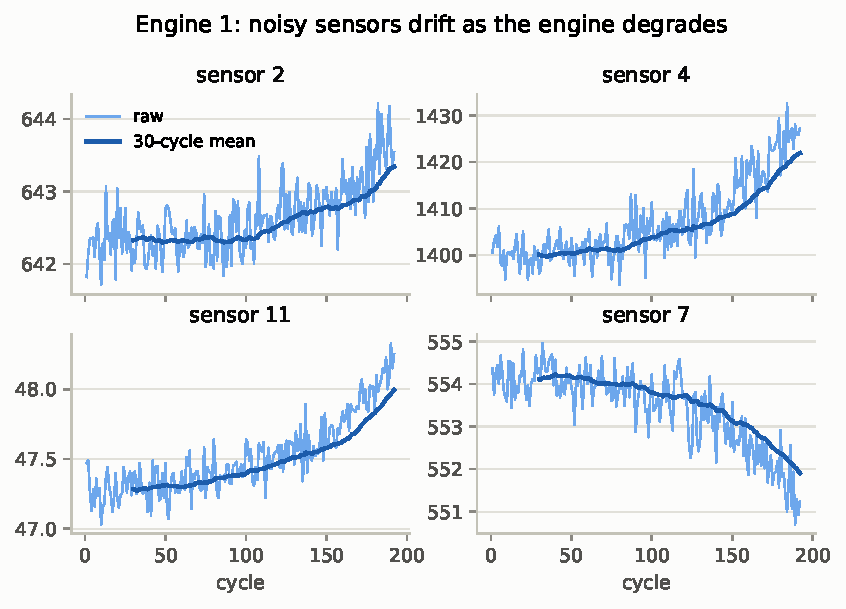
\includegraphics[width=0.8\textwidth]{eda_sensor_traces.pdf}
\caption{Four sensors of one engine. Single readings are noisy; a rolling mean shows the slow drift that is the
degradation.}
\end{figure}

Six sensors (\ConstantSensors{}) never change in FD001; they carry no information. The others drift as the
engine degrades, buried in noise. That is why the system computes features over a \emph{window} of recent
readings instead of looking at one reading.

\subsection{The cap on RUL}
Early in its life an engine is healthy, and its sensors look the same whether it has 300 or 200 cycles left.
Asking a model to tell those apart is asking it to predict noise. The usual convention for this dataset is to
cap the label: any RUL above \LabelCap{} is recorded as \LabelCap{}. Read it as ``healthy, at least \LabelCap{} cycles left''.
In the training data \EdaShareRowsAboveCap{}\% of rows are above the cap.

%=====================================================================
\section{The CS tooling}

\subsection{The shape of the system}
\begin{lstlisting}
replayer --HTTP--> ingest API --> [Kafka topic: readings] --> processor
                                                               |-> PostgreSQL (readings, scores, alerts)
                                                               |-> Redis (window per machine)
                                                               |-> model (ONNX Runtime, in-process)
                                                               '-> alert engine
dashboard <--REST + Server-Sent Events-- query API
\end{lstlisting}

\subsection{Java 21 and Spring Boot}
Spring Boot assembles an application from \emph{beans}: objects that Spring creates and wires together by
type. A class annotated \texttt{@RestController} becomes an HTTP endpoint; \texttt{@Configuration} classes
declare beans with \texttt{@Bean} methods; \texttt{@ConditionalOnProperty} turns a bean on or off from
configuration. That is how one jar runs as a ``direct'' pipeline (processing inside the request) or a
``kafka'' pipeline, by a single property. Java 21's \emph{virtual threads} let the replayer run one cheap
thread per engine.

\subsection{PostgreSQL and Flyway}
PostgreSQL stores readings, health scores and alerts. Flyway applies numbered SQL migrations
(\texttt{V1\_\_machines.sql}, \ldots) on startup, so the schema is versioned with the code. The key design
choice: the primary key of \texttt{readings} is \texttt{(machine\_id, cycle)}. Inserting the same reading
twice with \texttt{ON CONFLICT DO NOTHING} is harmless, which makes retries safe.

\subsection{Redis}
Redis is an in-memory key-value store. The processor keeps each machine's last \Window{} readings there
(\texttt{window:\{id\}}), so a restart does not forget them.

\subsection{Kafka}
Kafka is a durable, partitioned log. Producers append messages to a \emph{topic}; consumers read them at their
own pace and record how far they got (the \emph{offset}). A topic is split into \emph{partitions}; Kafka keeps
order only within one partition. Messages with the same \emph{key} go to the same partition, so keying by
machine id keeps each machine's readings in order while different machines are processed in parallel.

\begin{keyidea}{at-least-once delivery}
The consumer commits an offset only after it has processed the message. If it crashes in between, the message
is delivered again. So the processor must be \emph{idempotent}: processing a message twice must change
nothing. Primary keys on \texttt{(machine, cycle)} and the ``ignore late cycles'' rule make it so.
\end{keyidea}

\subsection{ONNX and ONNX Runtime}
ONNX is a file format for trained models. We train in Python (scikit-learn), export with \texttt{skl2onnx}, and
load the file in Java with ONNX Runtime. A \emph{parity test} checks that Java and Python give the same
prediction for the same input; without it you might ship a different model from the one you validated.

\subsection{Testing: JUnit, Testcontainers, pytest}
Unit tests check one class with hand-computed values. Integration tests start the whole application against a
real PostgreSQL, Redis and Kafka; Testcontainers starts them in Docker for the test, or the tests point at
local services when Docker is absent. pytest checks the Python invariants: no engine leaks between splits, the
features equal a slow reference, the metrics equal hand-computed values, the ONNX file equals sklearn.

\subsection{k6, Micrometer, Server-Sent Events}
k6 is a load generator scripted in JavaScript; it reports throughput and latency percentiles. Micrometer
exposes counters and timers from inside the service (readings ingested, processing lag, inference time).
Server-Sent Events (SSE) keep one HTTP response open and push named events down it; the dashboard listens
with \texttt{EventSource}.

%=====================================================================
\section{Classical machine learning}

\subsection{Supervised regression}
Given examples $(x_i, y_i)$, learn a function $f$ with $f(x) \approx y$ on \emph{new} examples. Here $x$ is the
feature vector of one machine at one cycle and $y$ its capped RUL.

\subsection{Features from a sliding window}
For each sensor we keep the last $W=\Window{}$ values $v_1, \dots, v_n$ ($n \le W$) and compute
\[
\bar v = \frac1n\sum v_k,\qquad
s = \sqrt{\frac1n\sum (v_k-\bar v)^2},\qquad
b = \frac{\sum (k-\bar k)(v_k-\bar v)}{\sum (k-\bar k)^2}.
\]
The mean $\bar v$ says where the sensor is, the standard deviation $s$ how noisy it is, and the slope $b$ how
fast it is moving.

\begin{keyidea}{the sliding window in O(1)}
Re-summing $W$ values for every new reading costs $O(W)$. Instead keep running sums $\sum v$, $\sum v^2$ and
$\sum k\,v$; when a value enters and one leaves, update the sums with a few additions and subtractions. Mean,
variance and slope follow from the sums in constant time. Two details make it correct in practice: subtract
an offset (the first value) so that sums of numbers near 9000 do not lose precision, and rebuild the sums from
the buffer every 1024 updates so rounding errors cannot accumulate.
\end{keyidea}

\subsection{Baselines}
Always compare with something trivial. The \emph{trivial} model predicts the mean training RUL for everyone;
its error is the ceiling any useful model must beat by a wide margin. \emph{Ridge regression} is a linear model
with a penalty on large weights; it is the simplest real model.

\subsection{Decision trees and gradient boosting}
A regression tree splits the data by questions like ``is the mean of sensor 11 above 47.6?'' and predicts the
average label in each leaf. One tree is crude. \emph{Gradient boosting} fits trees one after another; each new
tree predicts what the ensemble so far gets wrong (the residual), and is added with a small weight (the
learning rate). Hundreds of small trees make a strong, non-linear model. Its key knobs are the number of trees,
the learning rate, the tree depth and the fraction of rows each tree sees (subsample). Because the trees are
added in order, the model with the first $n$ trees is exactly the model you would get by training $n$ trees,
which makes choosing $n$ on validation cheap.

\subsection{Overfitting and validation}
A model can memorise its training data. To choose anything (the number of trees, the sensors, the alert
thresholds), measure on data the model did not train on: the \emph{validation} split. Keep a third split, the
\emph{test} split, untouched until the very end, so that the final number is not shaped by your choices.

%=====================================================================
\section{Deep learning, and why it is not used here}

\subsection{Neural networks in one page}
A neural network is a stack of layers; each computes $h = \sigma(Wx + b)$, a linear map followed by a
non-linear function $\sigma$. Training adjusts $W$ and $b$ by gradient descent on a loss (for regression, the
mean squared error), with gradients computed by backpropagation. For sequences there are dedicated
architectures: recurrent networks (LSTM, GRU) carry a state from one time step to the next; one-dimensional
convolutions slide learned filters along time; transformers let every step attend to every other step.

\subsection{Deep learning on C-MAPSS}
The RUL literature on this dataset includes many LSTM and CNN models that read a window of raw readings
and learn their own features. They can be competitive with a well-featured tree model, at the cost of more
hyper-parameters, more training time, more seeds needed to average out their variance, and a harder export and
parity story.

\subsection{Why gradient boosting here}
The question of this project is about sensors and systems, not about the best possible model. A tree ensemble
on explicit window features is fast to train (seconds to minutes), deterministic given a seed, exports cleanly
to ONNX, scores in \JavaUsPerPrediction{}\,\textmu s in Java, and its importance can be read per sensor, which
is exactly what the sensor question needs. A neural model would be a reasonable extension, evaluated under the
same split, seeds and budget.

%=====================================================================
\section{The method under test: sensor reduction}

\subsection{The question}
Every sensor is hardware, wiring and a failure mode. If 8 sensors predict RUL as well as 21, the service should
run on 8. The project asks this before building the final model, and answers it with a controlled experiment.

\subsection{The three arms}
\begin{itemize}
\item \textbf{all 21 sensors};
\item \textbf{15 informative sensors}: drop the constant ones (\InformativeSensors{} remain);
\item \textbf{8 ranked sensors}: the 8 sensors whose window mean has the largest absolute Spearman correlation with
RUL on the \emph{training} engines: \ReducedEightSensors{}.
\end{itemize}
Everything else is identical: split, window, label, model, hyper-parameters, the grid of tree counts, the
selection rule and the seeds. An experiment that changes two things at once cannot tell you which mattered.

\subsection{Non-inferiority}
``As good as'' needs a definition. We fixed a margin: the 8-sensor model may be worse by less than \Margin{}
cycle of mean test RMSE. That is a \emph{non-inferiority} hypothesis. Without a margin, any difference, however
tiny, would count as ``worse'', and any non-significant difference would be misread as ``the same''.

%=====================================================================
\section{Evaluation methodology}

\subsection{Group-aware splits}
Consecutive cycles of one engine are almost identical. If cycles of the same engine land in both training and
test, the model is tested on near-copies of its training data, and the score is a lie. So the split is by
engine: \SplitTrain{} training, \SplitVal{} validation and \SplitTest{} test engines, frozen in a JSON file, with a
test that fails if any engine appears twice.

\begin{keyidea}{how big is the lie?}
We measured it (post hoc). The same model, evaluated on a random split of \emph{rows}, reports
\RowsplitRmse{} cycles of RMSE. Evaluated honestly, on unseen \emph{engines}, it gets \MainGbrFullTwoOneTestRmse{}.
The leaky number is \RowsplitOptimismPct{}\% too optimistic.
\end{keyidea}

\subsection{Pre-registration}
Before the first main result existed, every choice was written into \texttt{model/config/experiment.json} and
committed: split, metric, window, cap, model, hyper-parameters, tree grid, selection rule, seeds, the hypothesis
with its margin, and the deployment rule. Pre-registration removes the temptation to change the recipe until the
result looks good. What was decided later is labelled \emph{post hoc} everywhere.

\subsection{Metrics: RMSE, and why not accuracy}
The headline is root mean squared error of RUL in cycles. The service turns RUL into a status, HEALTHY,
WARNING or CRITICAL, so we also report status accuracy, macro-F1 and CRITICAL recall. Accuracy misleads on an
imbalanced label: most rows are HEALTHY, so the trivial model scores \BaselineTrivialMeanFullTwoOneStatusAccPct{}\%
accuracy while catching no CRITICAL machine (recall \BaselineTrivialMeanFullTwoOneCriticalRecall{}). Macro-F1
averages the score over the three statuses, so it punishes ignoring the rare ones.

\subsection{Seeds and budget}
Random choices (which rows each tree sees) change the result a little. Each arm was trained with
\NSeeds{} seeds, and we report mean $\pm$ standard deviation. Every arm had the same budget: the same grid of tree
counts, chosen by the same rule on validation only.

\subsection{Read the test split once}
The test engines are scored once per finished run, at the configuration chosen on validation. If you look at the
test score and then change something, the test split has become a validation split, and you no longer have an
unbiased number.

%=====================================================================
\section{Build diary, block by block}

\subsection{Block 0: environment, data, exploration}
Installed a portable toolchain (JDK 21, Maven, PostgreSQL, Redis, Kafka, k6), downloaded FD001, checked it by
eye and by count: \EdaEngines{} engines, \EdaRows{} rows, contiguous cycles, no duplicates, six constant
sensors. Built the Spring Boot skeleton with a health check and the first migration.

\begin{mistake}{zero tests ran, and the build said success}
Maven's test runner only picks up classes named \texttt{*Test} by default; our integration tests are
\texttt{*IT}. The first ``green'' build ran nothing. Fix: include \texttt{*IT.java} explicitly, and always read
the test count, not just the word SUCCESS.
\end{mistake}

\begin{mistake}{servers that died with the session}
Databases started from a tool call died when the session ended, and one received a Ctrl+C meant for its parent.
Fix: start them detached, in their own process group, from a script; stop processes only by PID.
\end{mistake}

\subsection{Block 1: ingest, storage, replayer, frozen split}
\texttt{POST /api/readings} validates and stores; the replayer streamed all 100 engines; the database held
exactly as many rows as the file, and a second replay changed nothing. The engine split was frozen with a leak
test.

\subsection{Block 2: features, pre-registration, baselines}
\begin{mistake}{fast features that were wrong}
The first vectorised feature code used running sums on raw values near 9000. Variance computed as
$\overline{v^2} - \bar v^2$ lost almost all its digits, and the test against a slow reference failed. Fix: compute
each window directly (two passes) in Python, and in Java keep sums relative to an offset and resynchronise them
periodically.
\end{mistake}

\begin{mistake}{an arm named after the wrong count}
The ``informative'' arm was planned as 14 sensors, but the rule (standard deviation above $10^{-6}$ on training
engines) keeps sensor 6, which is nearly but not exactly constant: 15 sensors. The arm was renamed before any
result, instead of quietly changing the rule to match the name.
\end{mistake}

\subsection{Block 3: the main experiment}
Nine runs (three arms, three seeds) went through a resumable queue that skips finished runs and writes a status
file, launched detached after profiling one short fit. The result is in Section~\ref{sec:read}.

\begin{mistake}{the double-precision model that could not run}
The plan was to export the trees with double-precision input, so that no threshold is rounded. ONNX Runtime's
tree operator cannot produce double output, so the session failed to load. Fix: float32 input, with the error it
introduces measured and bounded by the parity test.
\end{mistake}

\begin{mistake}{trust, then verify, a surprising result}
Before writing anything, every checkpoint was reloaded, every test score recomputed from it, and the 8-sensor
columns rebuilt from scratch. The surprising identity of the 15- and 21-sensor models turned out to be exact
and explainable: no tree ever splits on a constant sensor (\AuditConstSplits{} splits).
\end{mistake}

\subsection{Block 4: alerts}
\begin{mistake}{an alert rule that fired on noise}
The first trend rule (RUL fell more than \OriginalTrendDrop{} over \OriginalTrendWindow{} readings) compared two
single predictions. Predictions jitter by several cycles from one reading to the next, so the rule kept opening and
closing WARNING alerts: only \AlertOriginalPass{} of \SplitVal{} validation engines produced the required single
WARNING then single CRITICAL. Fix, designed on validation only: fit a least-squares slope over
\AlertTrendWindow{} readings, require a full window before any alert, and confirm once on the test engines
(\AlertReplayTestEnginesPassing{} of \AlertReplayTestEngines{}).
\end{mistake}

\begin{mistake}{the first score, counted twice}
To design the rule quickly, the alert engine was re-implemented in Python and checked against the Java service
engine by engine. Three engines disagreed. The cause was in Java: after a restart the engine rebuilt its recent
scores from the database, which already contained the score being evaluated, so that score was counted twice.
\end{mistake}

\begin{mistake}{tests that poisoned the dev database}
Integration tests wrote windows into the same Redis database the dev service used. A later replay found machine
9 ``already at cycle 40'' and ignored its first 40 readings as late. Fix: tests use their own Redis database and
their own Kafka topic.
\end{mistake}

\subsection{Block 5: Kafka, crash safety, error analysis}
\begin{mistake}{saving the window before the score}
The processor saved the machine's window to Redis \emph{before} storing the score. A crash between the two would
make the redelivered reading look late, and its score would never be written. Fix: save after the score and
alerts; on any failure, drop the in-memory window so the retry starts from the last saved state.
\end{mistake}

\begin{mistake}{deleting a topic killed the broker}
On Windows, Kafka cannot rename the folder of a deleted topic while files in it are open, and it shuts itself
down. Fix: never delete topics in experiments; use a fresh topic name per run.
\end{mistake}

The kill-and-restart experiment then passed: all \RestartFileRows{} readings stored and scored exactly once, scores
equal to an uninterrupted run within \RestartMaxDiff{}, and alerts identical to an uninterrupted run on every
machine.

\subsection{Block 6: dashboard, load test, write-up}
\begin{mistake}{a demo that showed nothing}
The dashboard said ``live'' but showed no predictions. A reset script had deleted the database rows but not the
Redis windows: \texttt{redis-cli} on Windows prints keys with a carriage return, so the shell loop deleted
nothing, and every reading was correctly ignored as late. Fix: one reset script that clears both stores and
asserts nothing is left.
\end{mistake}

%=====================================================================
\section{How to read the results}\label{sec:read}

\subsection{The pre-registered answer}
\begin{center}
\resizebox{\textwidth}{!}{\begin{tabular}{lrrrrrrrr}
\toprule
Method & Seeds & Test RMSE & Test MAE & NASA score & Status acc. & Macro-F1 & CRITICAL recall & Official RMSE \\
\midrule
trivial (train mean), all 21 sensors & 1 & 41.58 $\pm$ 0.00 & 36.98 $\pm$ 0.00 & 302.35 $\pm$ 0.00 & 0.717 & 0.278 & 0.000 & 41.97 $\pm$ 0.00 \\
ridge regression, all 21 sensors & 1 & 18.78 $\pm$ 0.00 & 14.26 $\pm$ 0.00 & 7.28 $\pm$ 0.00 & 0.850 & 0.700 & 0.640 & 19.45 $\pm$ 0.00 \\
ridge regression, 8 ranked sensors & 1 & 20.86 $\pm$ 0.00 & 15.61 $\pm$ 0.00 & 9.21 $\pm$ 0.00 & 0.849 & 0.695 & 0.616 & 21.33 $\pm$ 0.00 \\
gradient boosting, all 21 sensors & 3 & 12.99 $\pm$ 0.07 & 9.40 $\pm$ 0.09 & 2.86 $\pm$ 0.04 & 0.921 & 0.845 & 0.933 & 13.22 $\pm$ 0.12 \\
gradient boosting, 15 informative sensors & 3 & 12.99 $\pm$ 0.07 & 9.40 $\pm$ 0.09 & 2.86 $\pm$ 0.04 & 0.921 & 0.845 & 0.933 & 13.22 $\pm$ 0.12 \\
gradient boosting, 8 ranked sensors & 3 & 15.56 $\pm$ 0.06 & 11.15 $\pm$ 0.07 & 4.35 $\pm$ 0.07 & 0.913 & 0.832 & 0.935 & 15.35 $\pm$ 0.27 \\
\bottomrule
\end{tabular}
}
\end{center}
All 21 sensors: \pmsd{\MainGbrFullTwoOneTestRmse}{\MainGbrFullTwoOneTestRmseStd} cycles RMSE. The 8 ranked sensors:
\pmsd{\MainGbrReducedEightTestRmse}{\MainGbrReducedEightTestRmseStd}. The gap is \HypGap{} cycles, larger than the
\Margin{}-cycle margin, so the hypothesis is rejected and the service ships the 21-sensor model. Read the
$\pm$ as the spread over seeds, not as a confidence interval.

\subsection{What the post hoc ablations add}
\begin{itemize}
\item \textbf{Which 8 matters.} The ranked 8 are highly redundant (mean pairwise correlation
\RedundancyReducedEight{}). Random sets of 8 do better on average (\RandomEightTestRmse{}), the 8
\emph{lowest}-ranked sensors land at \PosthocGbrWorstEightTestRmse{}, and forward selection on validation reaches
\PosthocGbrGreedyEightTestRmse{}, within \GreedyEightGap{} of the full model.
\item \textbf{The recipe matters as much.} Changing the window from 30 to 60 readings improves the 21-sensor
model by \WindowEffectFullTwoOne{} cycles, about the size of the sensor effect. The verdict holds in every
setting tried, but its size depends on the recipe.
\end{itemize}

\begin{keyidea}{a negative result with a positive lesson}
The pre-registered experiment says ``no''. The ablations say why. Ranking sensors one at a time picks sensors that
repeat each other. Fewer sensors can work if they are chosen together. That is a hypothesis for a new
pre-registered experiment, not a conclusion of this one.
\end{keyidea}

\subsection{Errors by hand}
Of \EaTestRows{} test rows, \EaMisclassifiedRows{} get the wrong status, always a neighbouring one. Looking at
\EaInspected{} of them on whole-engine plots: \EaAmbiguous{} ambiguous, \EaMislabeled{} mislabeled, \EaModel{}
real errors. The real errors come in four shapes. The model lags on engines that fail fast, runs early near the
end of long-lived engines, jitters, and sometimes sticks at a tree leaf near 60.

%=====================================================================
\section{Interview questions, with answers}
\begin{enumerate}[leftmargin=*]
\item \textbf{Walk me through one reading, end to end.} Validated, inserted with \texttt{ON CONFLICT DO NOTHING},
published to Kafka keyed by machine and acknowledged, then consumed. The machine's window is updated in $O(1)$,
63 features feed the ONNX model, and the score is stored. The alert engine evaluates it, the window is saved to
Redis, and SSE pushes the update to the dashboard.
\item \textbf{The same reading arrives twice? Out of order?} Twice: the primary key makes the insert a no-op and
the processor sees a cycle that is not newer, so it is ignored. Out of order: a late cycle is ignored and
counted; a gap is accepted and logged.
\item \textbf{The processor crashes. What is lost?} Nothing. Offsets are committed after processing, the window is
saved after the score, and every write is idempotent. The kill-and-restart test shows identical scores and alerts.
\item \textbf{10,000 machines?} Partitions bound processing parallelism: add partitions and processor instances.
PostgreSQL writes are next: batch score inserts and partition \texttt{readings} by time. Redis is about 6 KB per
machine. The SSE stream must be sampled.
\item \textbf{Why PostgreSQL, and when would you switch?} The hot window is in Redis, and the rest is relational
(alerts with state). Switch, or add TimescaleDB, when retention by time or wide time-range scans dominate.
\item \textbf{Deploy a new model without downtime?} Export, run the parity test, ship the jar, roll the
instances. Every score stores its model version, so the two versions can be compared side by side.
\item \textbf{How do you know Java matches Python?} A parity test on \ParityRows{} real test rows within
$10^{\CfgParityTolExp}$, plus a feature fixture within $10^{\CfgFeatureTolExp}$.
\item \textbf{Which index did you add, and why?} A partial index on open alerts; the primary key
\texttt{(machine\_id, cycle)} already serves every chart query.
\item \textbf{What causes the p99?} See the load-test report: what the slowest requests wait on is measured,
not guessed.
\item \textbf{Why is accuracy not your headline?} Because a model that always says HEALTHY scores
\BaselineTrivialMeanFullTwoOneStatusAccPct{}\%.
\item \textbf{What would you do differently?} Pre-register the sensor \emph{selection method} as an arm of its own,
and choose the window on validation before the main comparison.
\end{enumerate}

%=====================================================================
\section{Glossary}
\begin{description}[leftmargin=2.2cm,style=nextline]
\item[Ablation] Removing or changing one part of a recipe to see how much it matters.
\item[At-least-once] A delivery guarantee: a message may arrive more than once, never zero times.
\item[Baseline] A simple model every real model must clearly beat.
\item[C-MAPSS] NASA's turbofan simulator and its published run-to-failure datasets.
\item[Cap (RUL)] Recording every RUL above a limit as the limit (\LabelCap{} here).
\item[Consumer group] Kafka consumers sharing the work of reading a topic; each partition goes to one member.
\item[Dead-letter topic] Where messages that fail repeatedly are parked for a human.
\item[Flyway] A tool that applies versioned SQL migrations.
\item[Gradient boosting] An ensemble of small trees, each fitted to the errors of the ones before.
\item[Group-aware split] A split that keeps all samples of one source (here, one engine) on one side.
\item[Hysteresis] Requiring a margin beyond a threshold before a condition counts as cleared, so it cannot flap.
\item[Idempotent] Doing it twice has the same effect as doing it once.
\item[Leak] Information from the test set reaching training or selection.
\item[Macro-F1] The F1 score averaged equally over classes.
\item[Non-inferiority] ``Not worse by more than a fixed margin.''
\item[Offset] A consumer's position in a Kafka partition.
\item[ONNX] An open file format for trained models.
\item[Parity test] A test that two implementations give the same output on the same input.
\item[Post hoc] Decided after seeing results.
\item[Pre-registration] Writing down the whole recipe before seeing any result.
\item[RMSE] Root mean squared error: the typical size of an error, in the label's units.
\item[RUL] Remaining useful life, in cycles.
\item[Seed] The number that fixes a run's random choices.
\item[SSE] Server-Sent Events: a one-way stream of named events over HTTP.
\item[Testcontainers] A library that starts real dependencies in Docker for a test.
\end{description}

\end{document}
